\chapter{Testare și Validare}
\pagestyle{fancy}

\section{Testare backend}
Pentru partea de backend, s-a realizat testare automată a API-urilor, utilizând Swagger. 
Conform definiției de pe Wikipedia pentru API~\cite{API}, este o interfață de programare a aplicației, care permite mai multor dispozitive să comunice între ele. \\
Așadar, trebuie să ne asigurăm că informațiile transmise bidirecțional sunt corecte, atât din punct de vedere al URL-ului utilizat (acesta este modul în care se va face legătura între backend și frontend), cât și din punct de vedere al răspunsului și formatul acestuia.

\subsection{Testare login cu crendențiale greșite}
În cazul încercării de logare în aplicație când utilizatorul introduce credențialele greșite, răspunsul va fi sugestiv și nu va fi logat în aplicație, după cum se poate vedea în figurile \ref{fig:loginWrong1} și \ref{fig:loginWrong2}.
\begin{figure}[H]
	\centering
	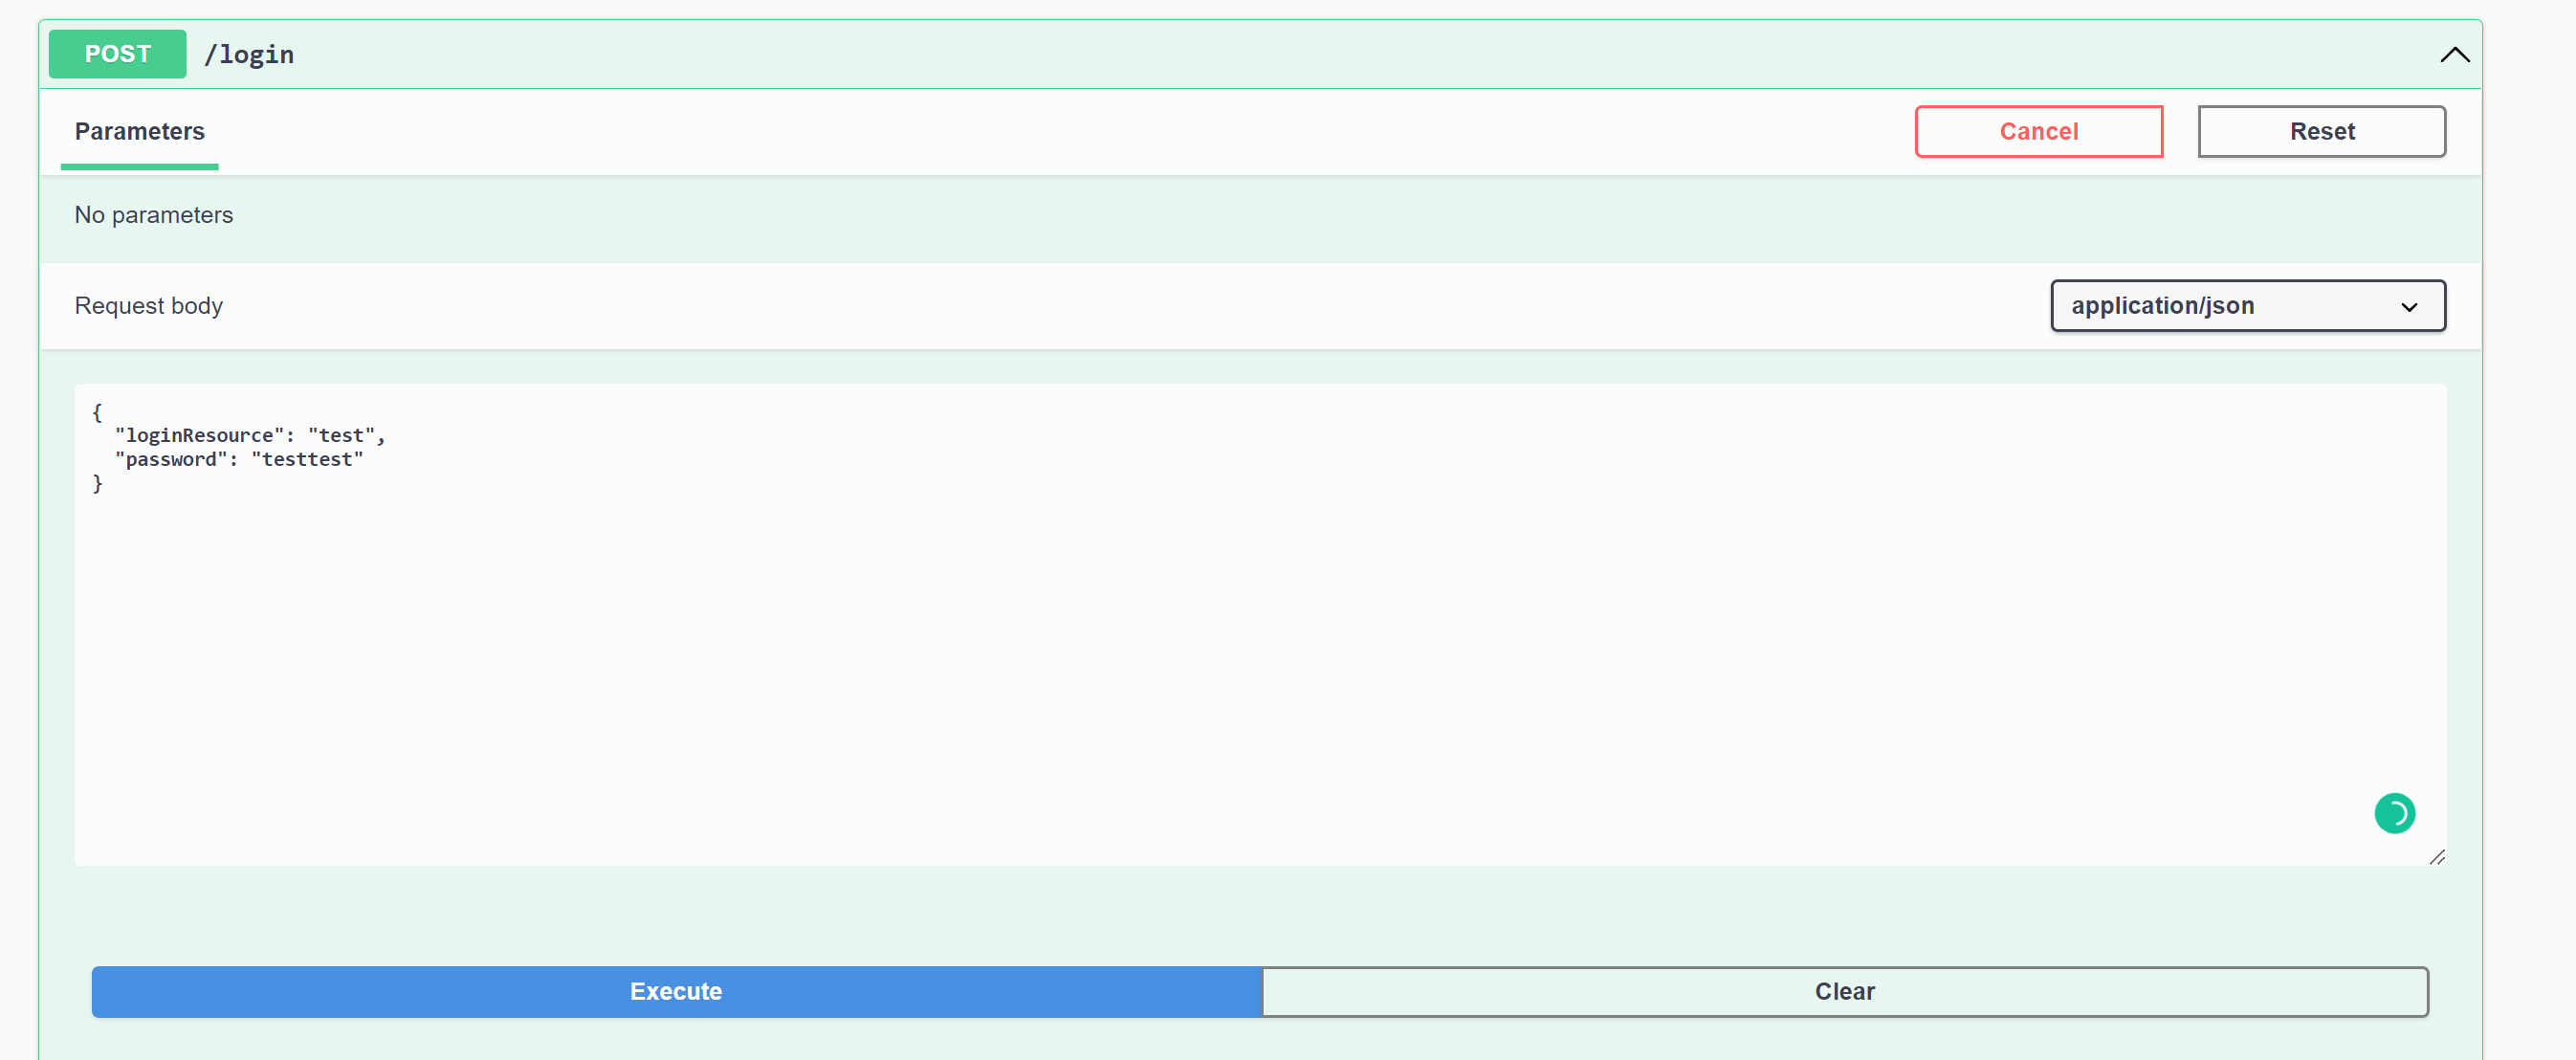
\includegraphics[width=100mm, scale=2]{figs/loginWrong1.png}
    \caption{Request - Login cu credențiale greșite}
	\label{fig:loginWrong1}
\end{figure}

\begin{figure}[H]
	\centering
	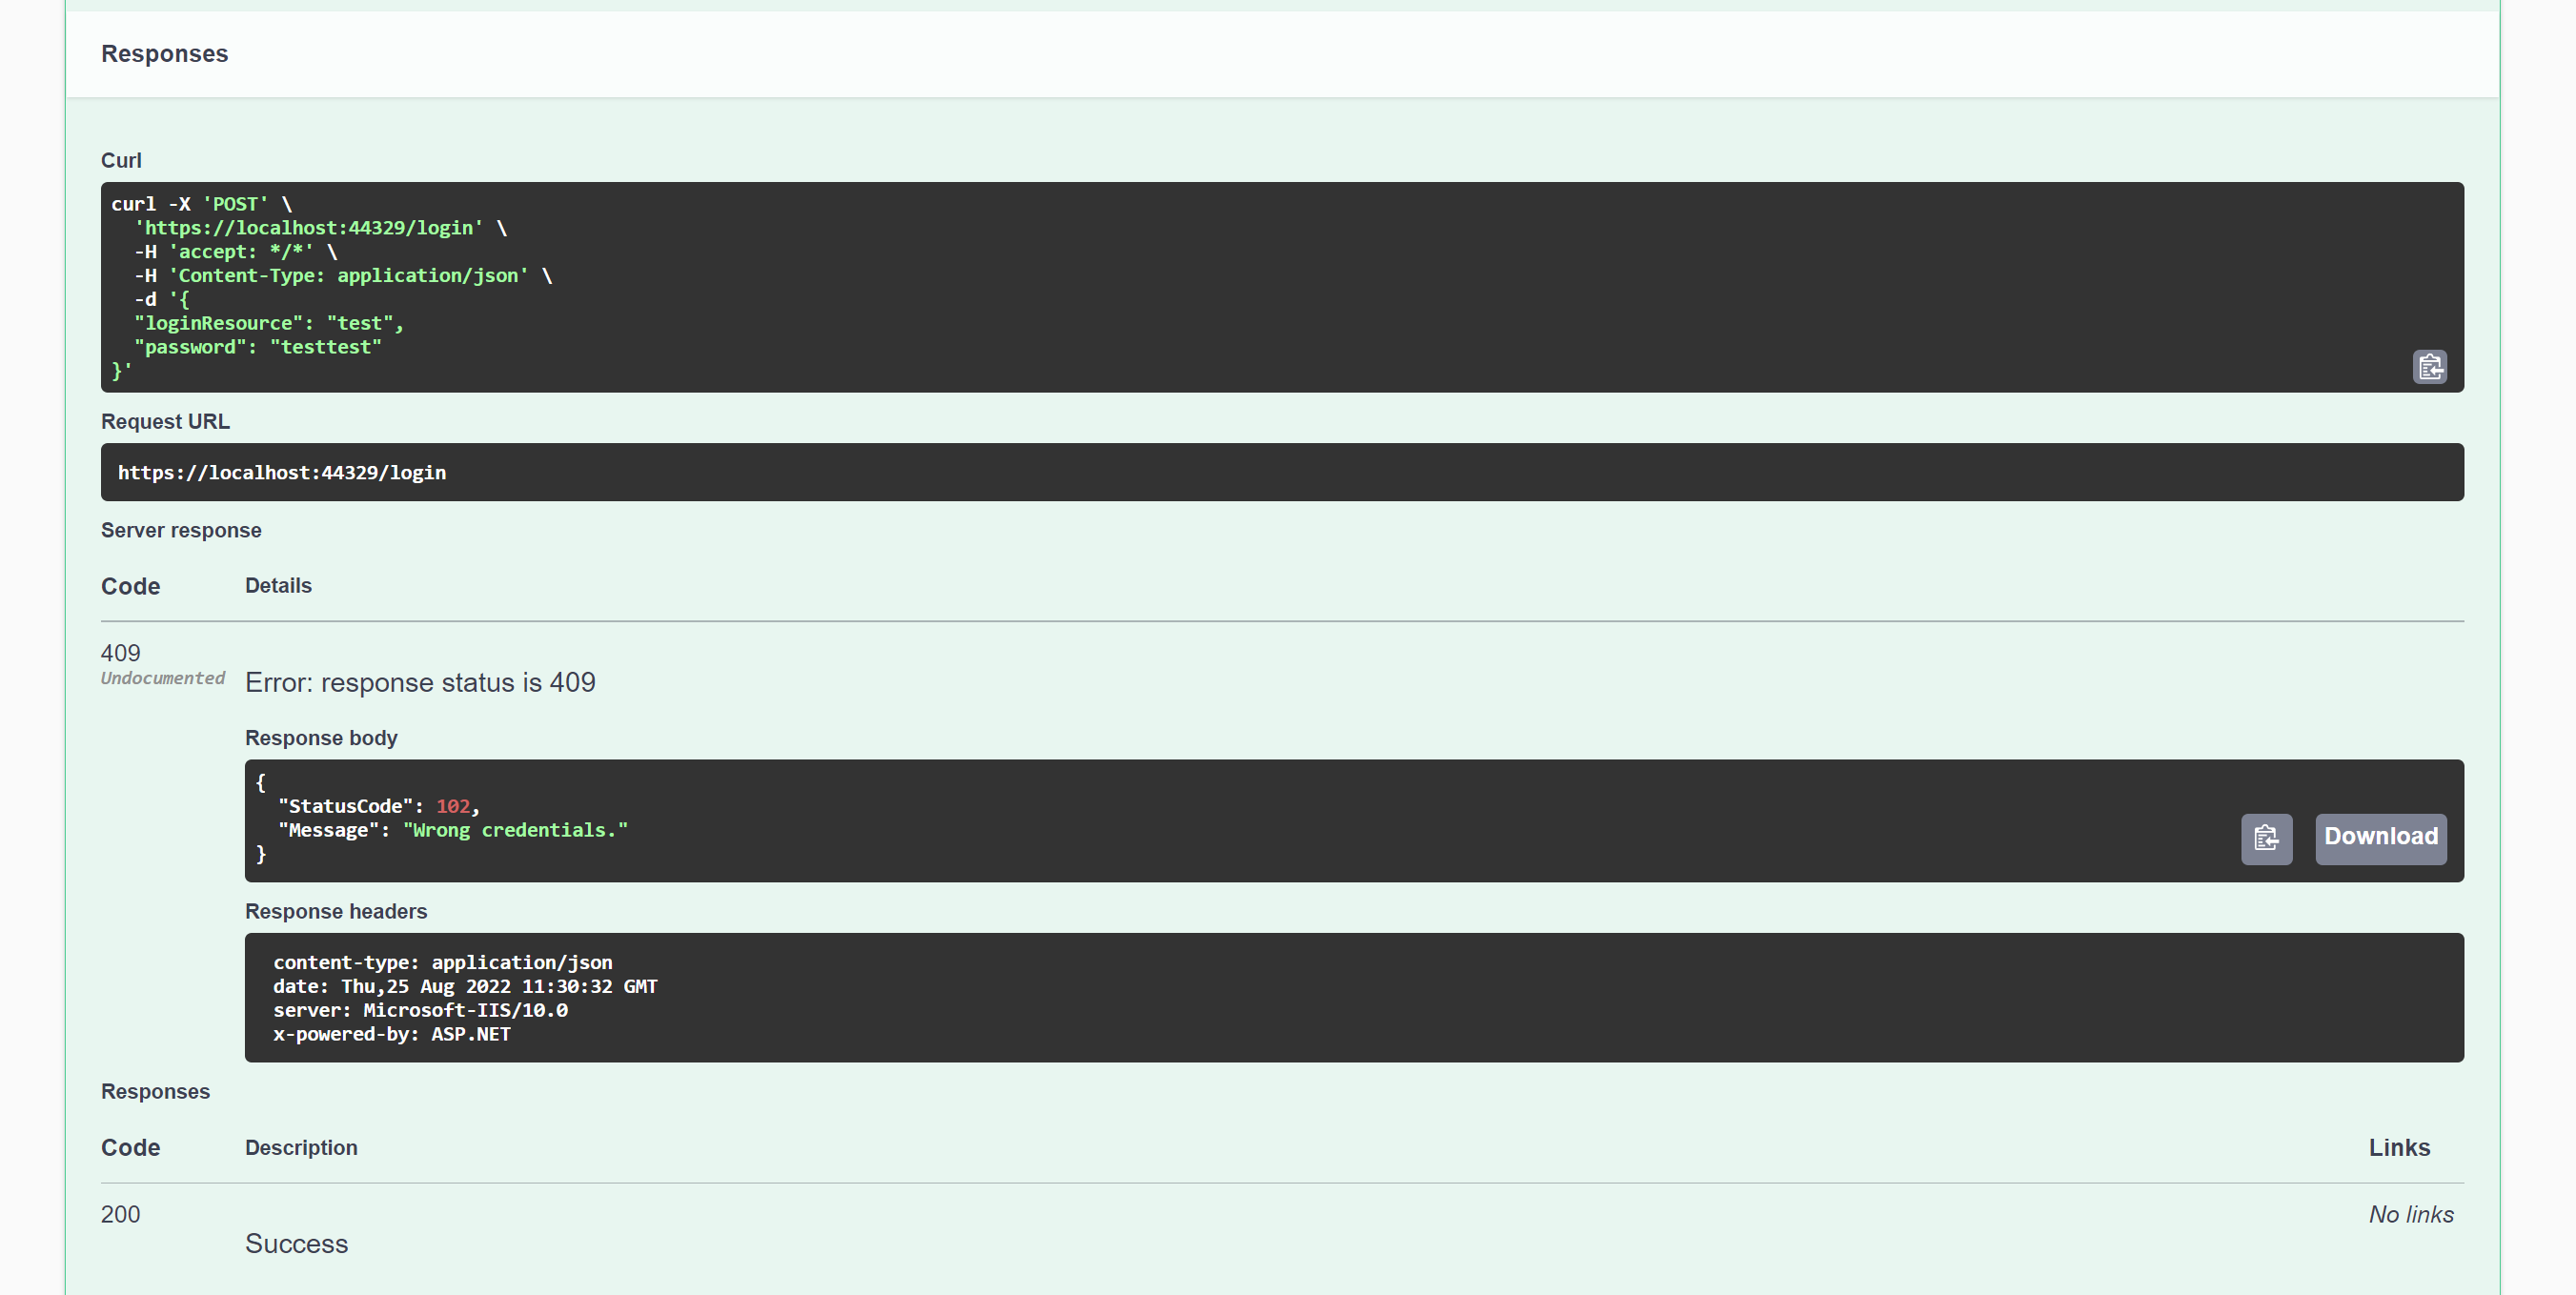
\includegraphics[width=100mm, scale=2]{figs/loginWrong2.png}
    \caption{Response - Login cu credențiale greșite}
	\label{fig:loginWrong2}
\end{figure}

\subsection{Testare login cu crendențiale corecte}
În cazul încercării de logare în aplicație când utilizatorul introduce credențialele corecte, răspunsul trimis la frontend va fi compus din Id-ul userului pentru a fi salvat în context și token-ul JWT generat, după cum se poate vedea în figurile \ref{fig:login1} și \ref{fig:login2}.

\begin{figure}[H]
	\centering
	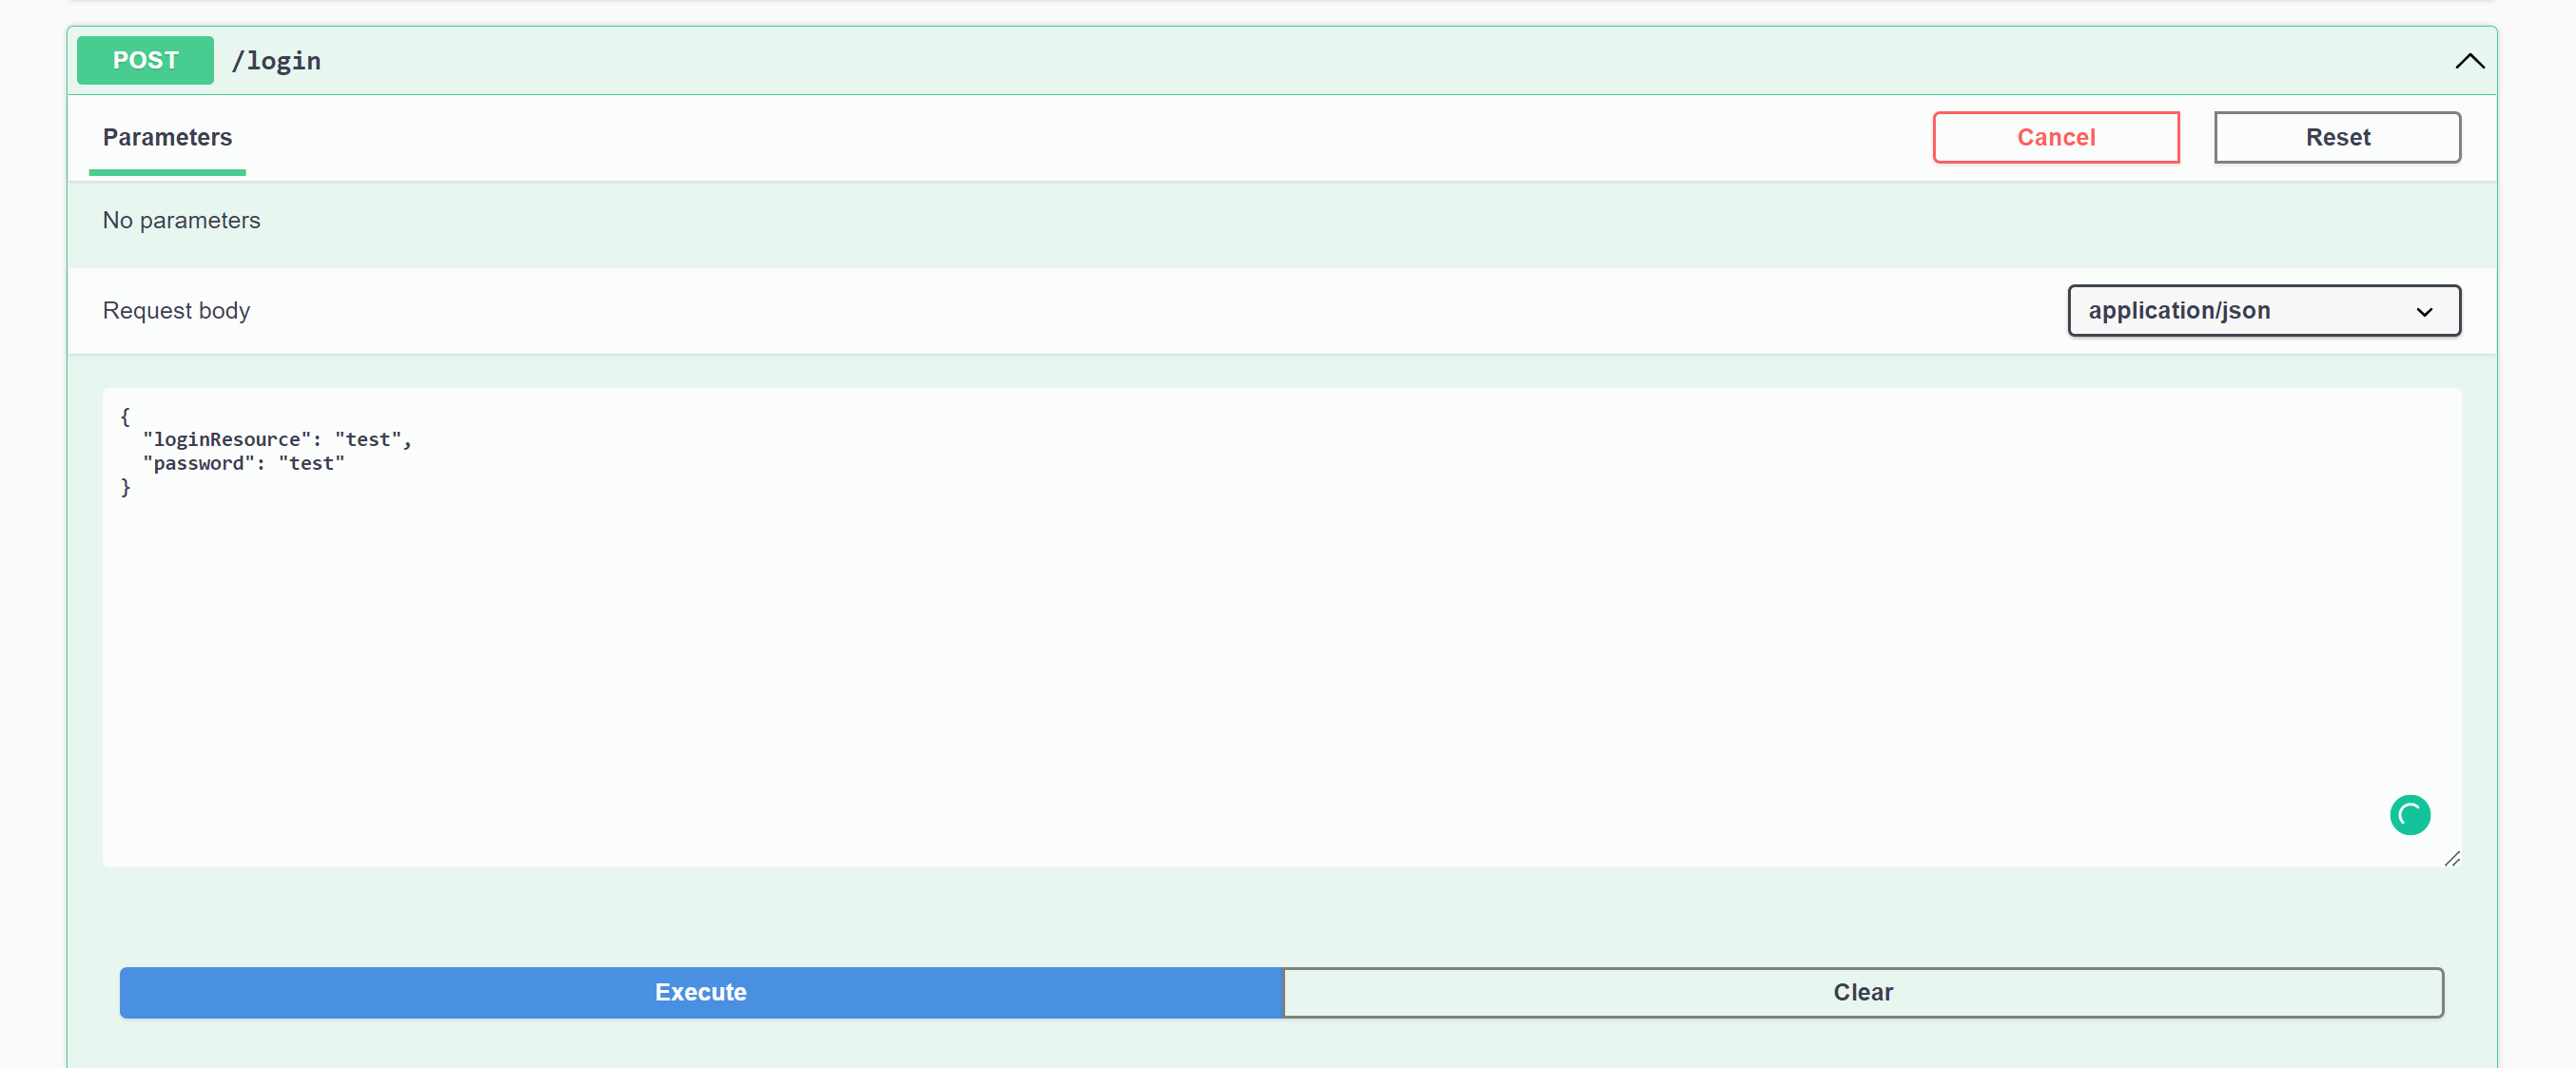
\includegraphics[width=100mm, scale=2]{figs/login1.png}
    \caption{Request - Login cu credențiale corecte}
	\label{fig:login1}
\end{figure}

\begin{figure}[H]
	\centering
	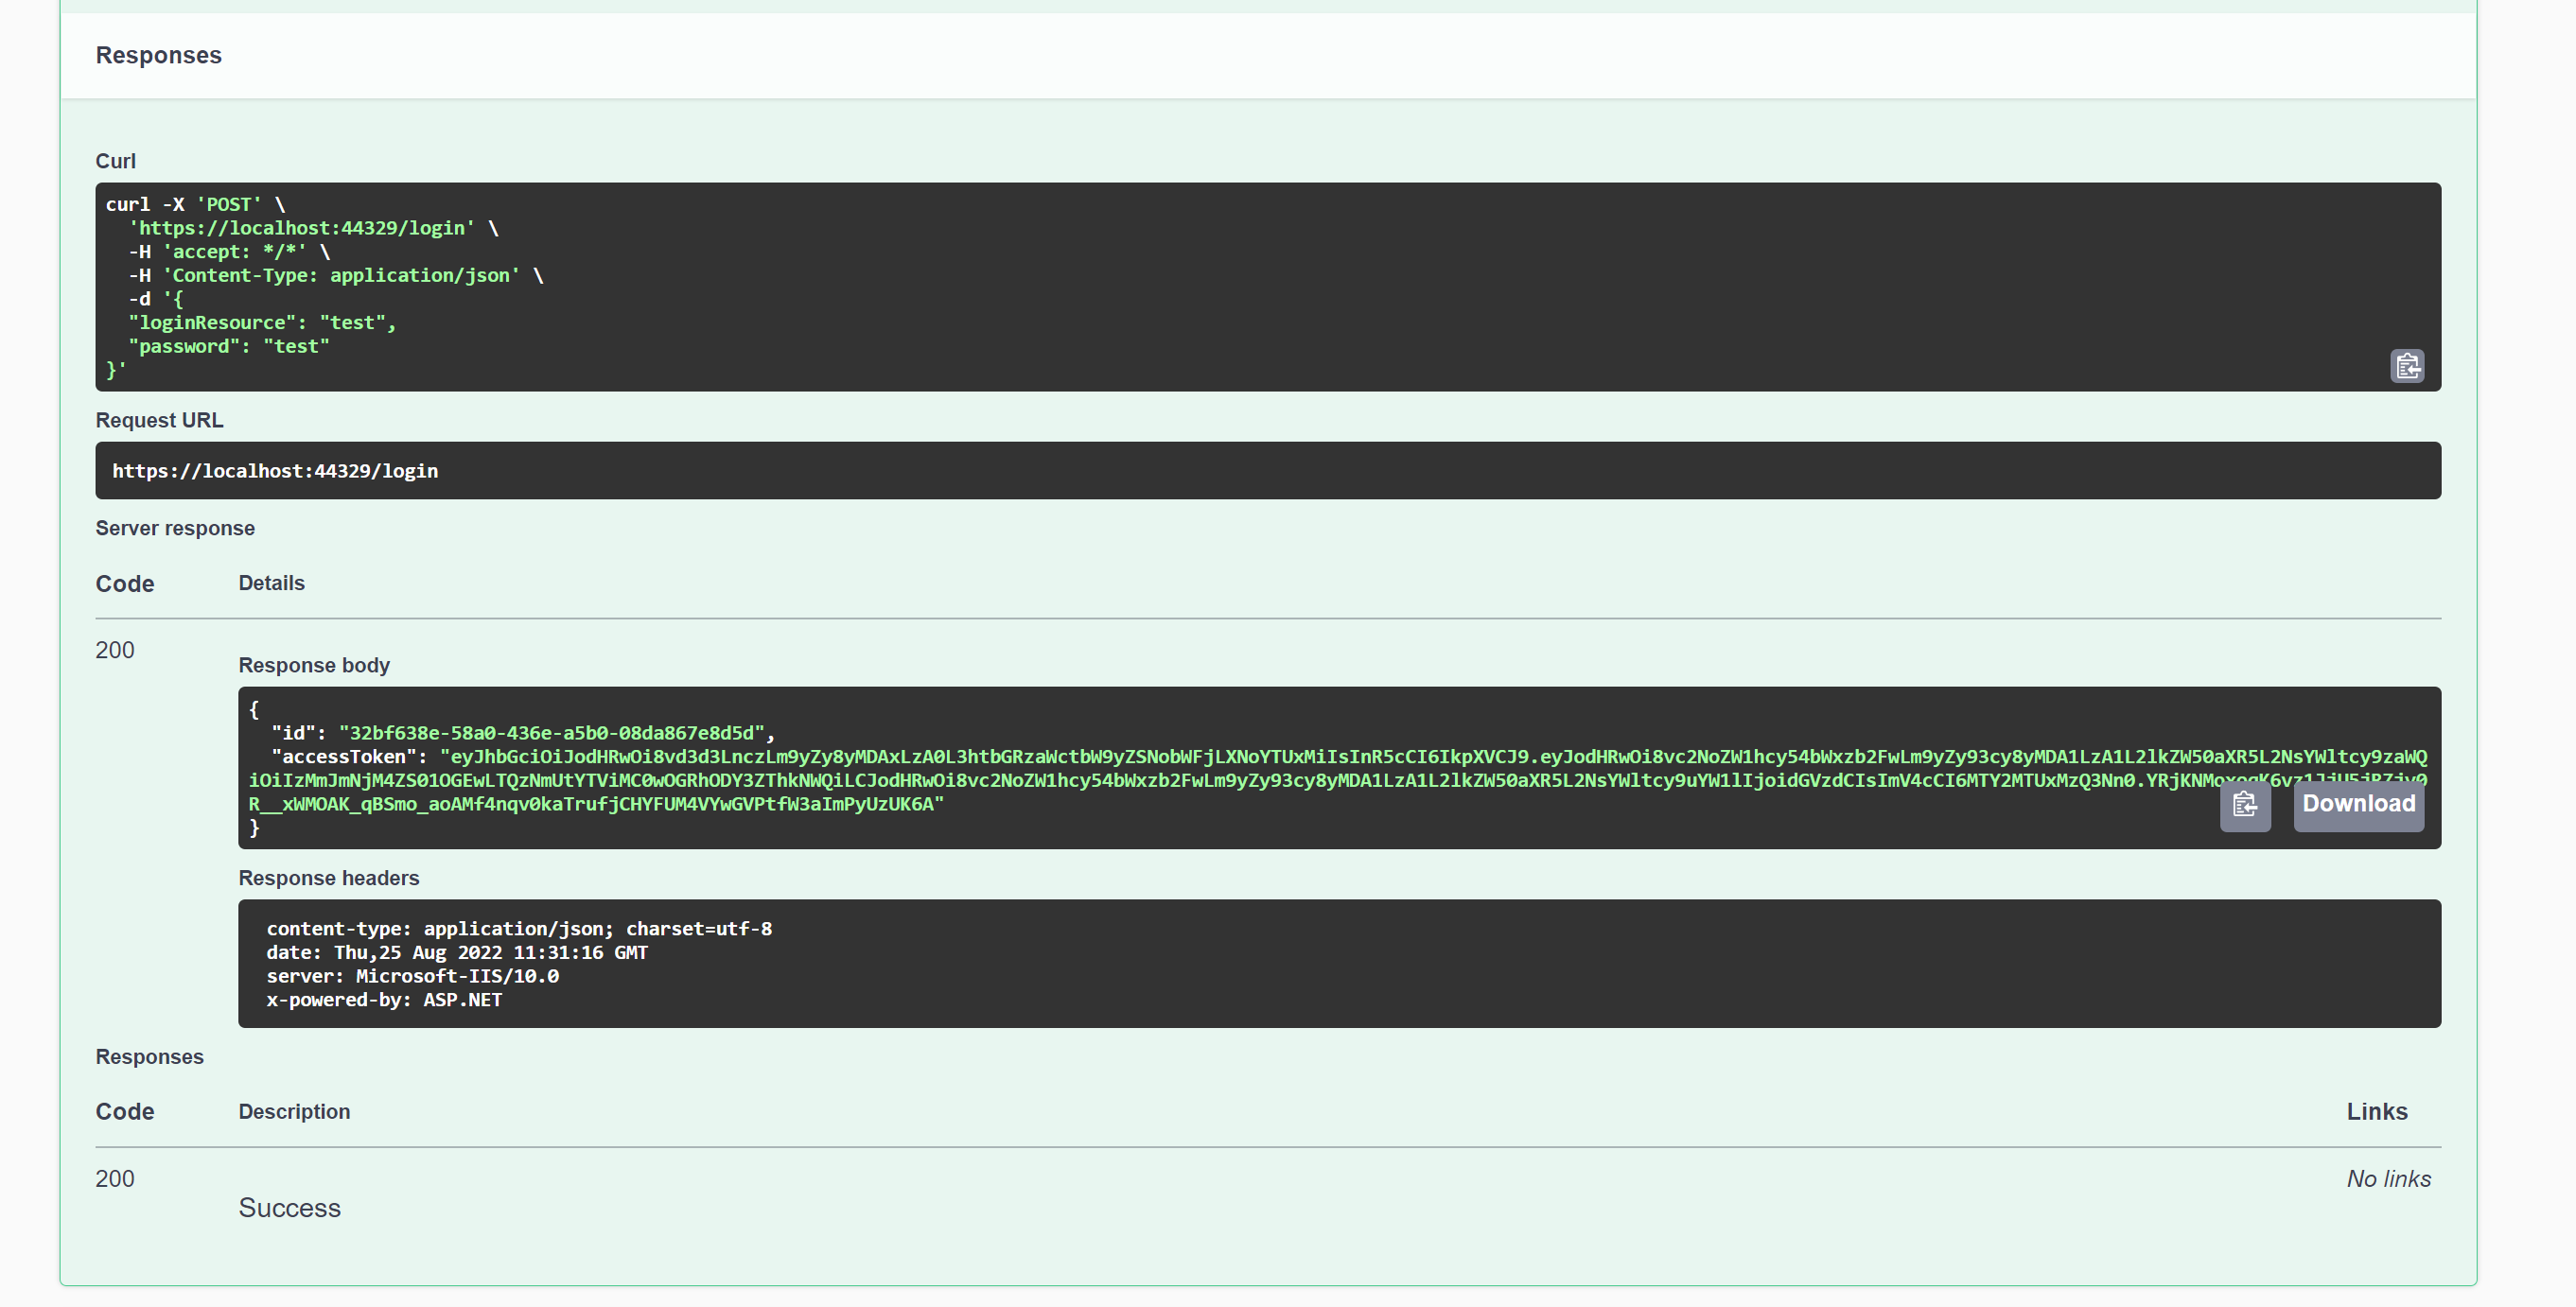
\includegraphics[width=100mm, scale=2]{figs/login2.png}
    \caption{Response - Login cu credențiale corecte}
	\label{fig:login2}
\end{figure}
\subsection{Testare editare detalii utilizator când un câmp este gol}
În cazul încercării de editare a detaliilor utilizatorului când un câmp este gol, deși ar trebui să conțină informație sub formă de string, răspunsul va fi generat de constrângerea validatorului creat cu ajutorul Fluent Validation,
după cum se poate vedea în figurile \ref{fig:editWrong1} și \ref{fig:editWrong2}.
\begin{figure}[H]
	\centering
	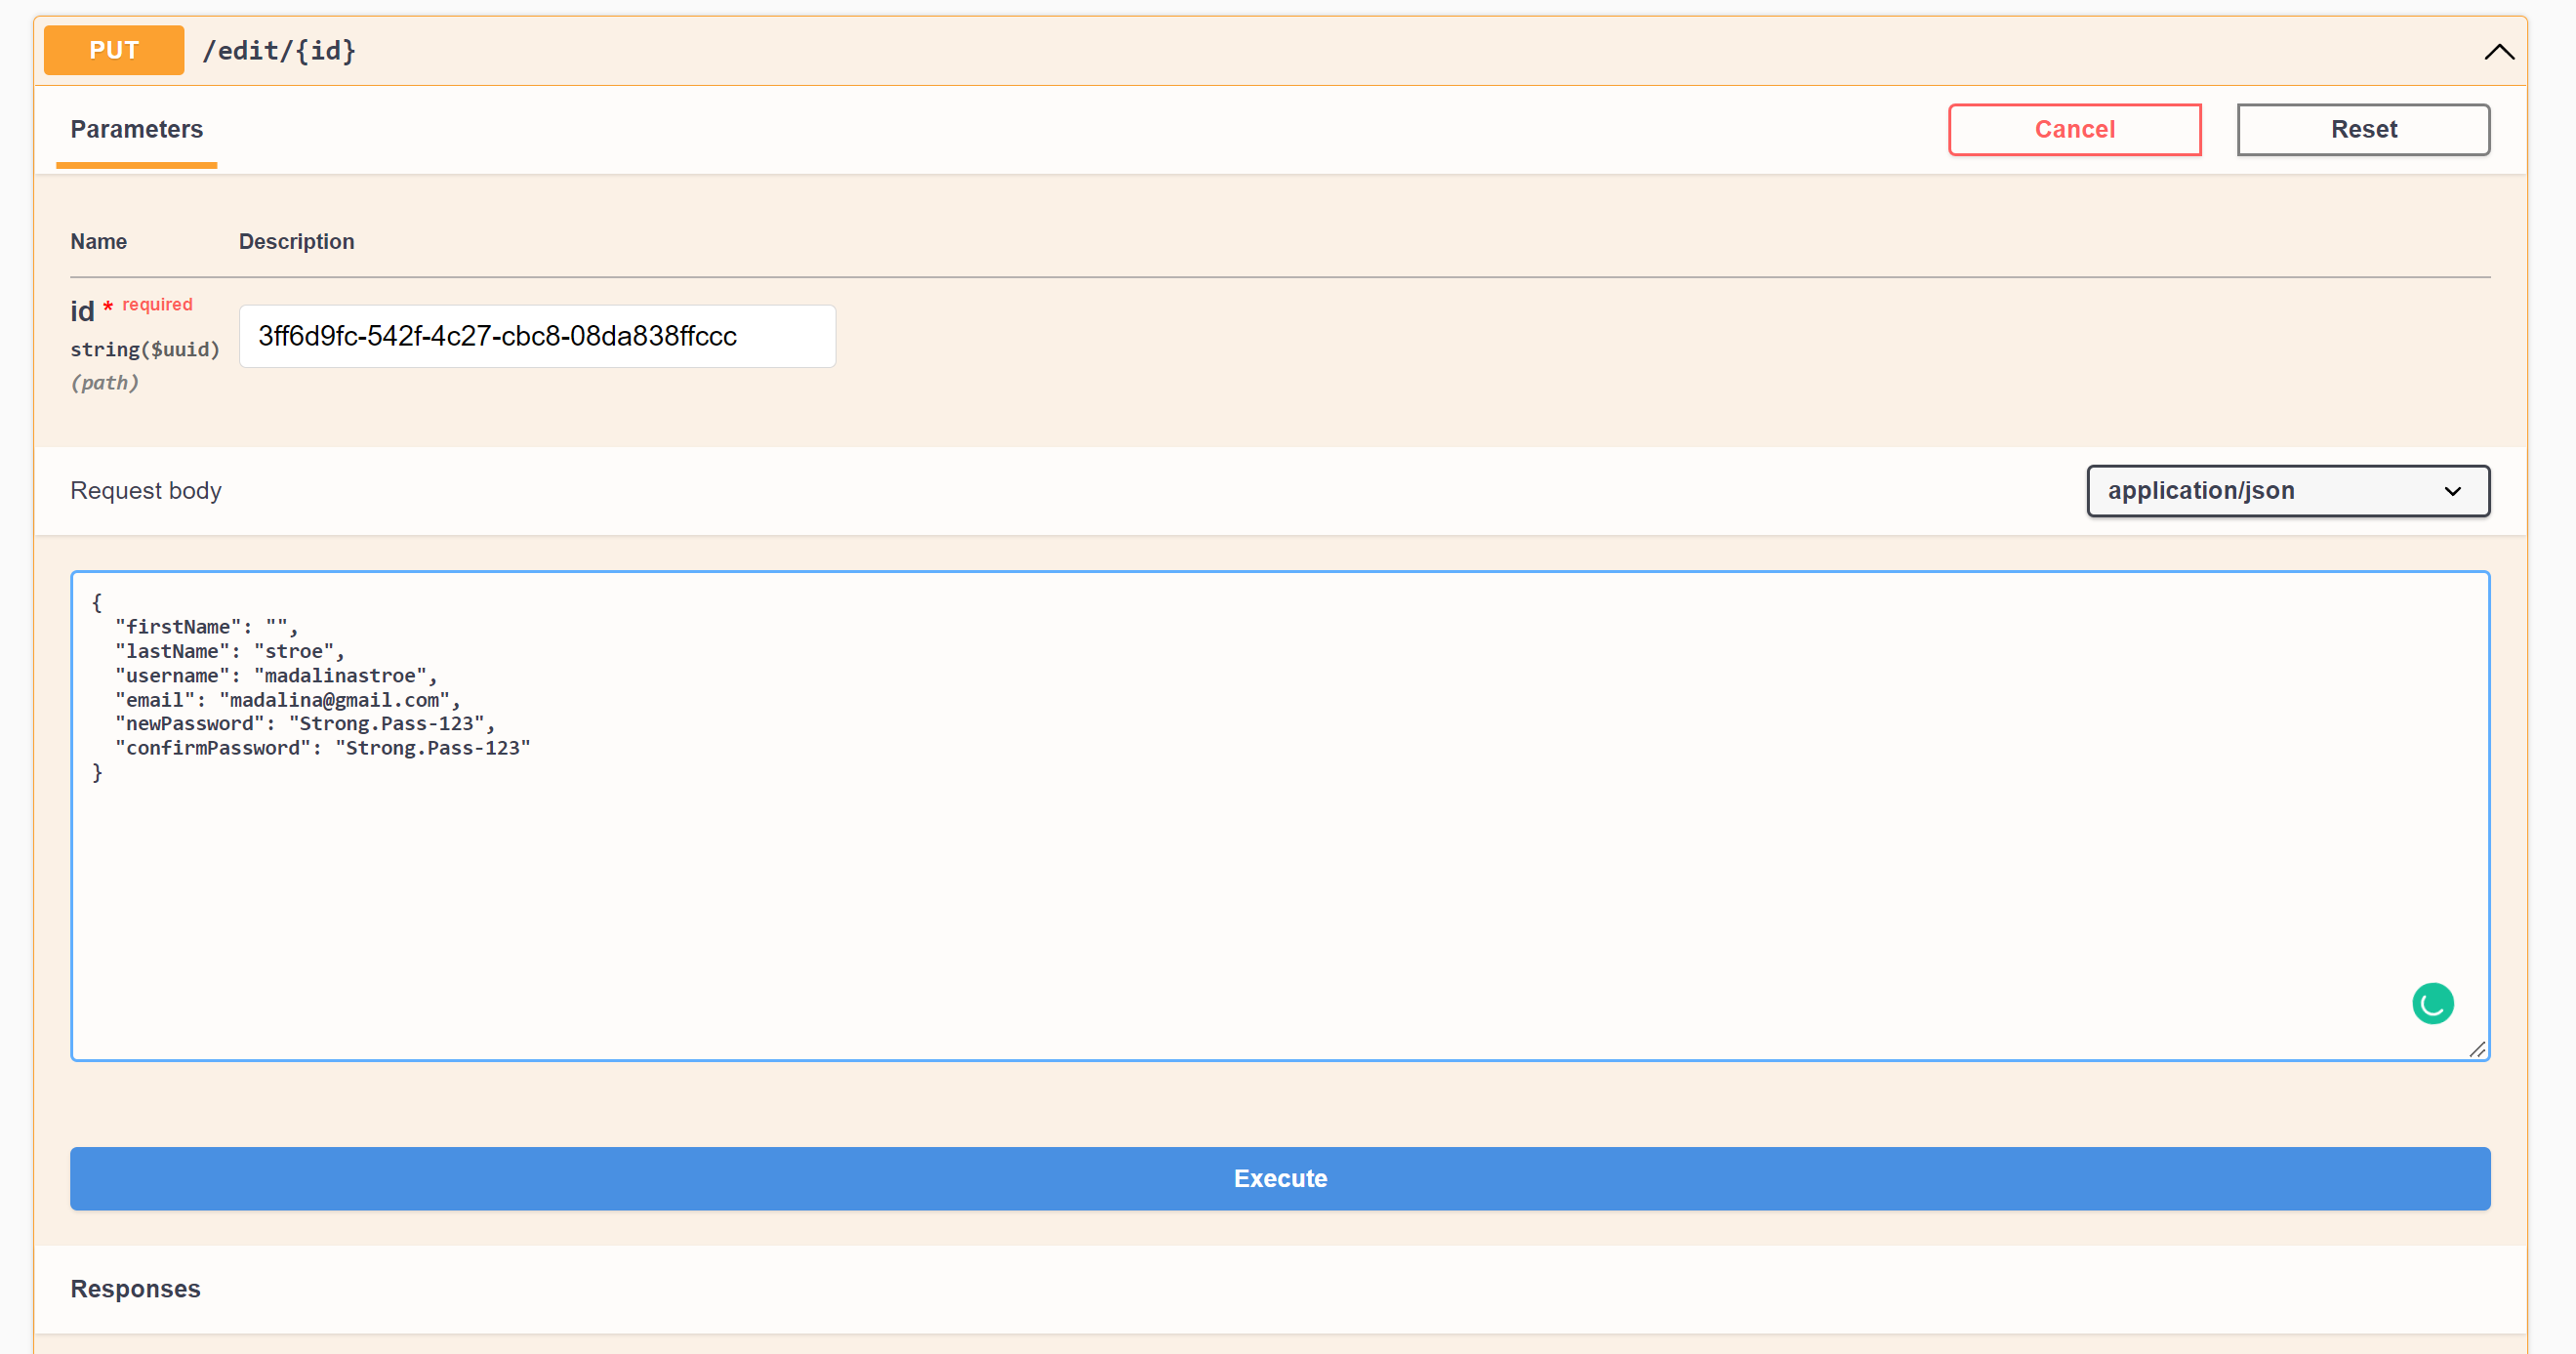
\includegraphics[width=100mm, scale=2]{figs/editWrong1.png}
    \caption{Request - Editare detalii personale când un câmp este gol}
	\label{fig:editWrong1}
\end{figure}

\begin{figure}[H]
	\centering
	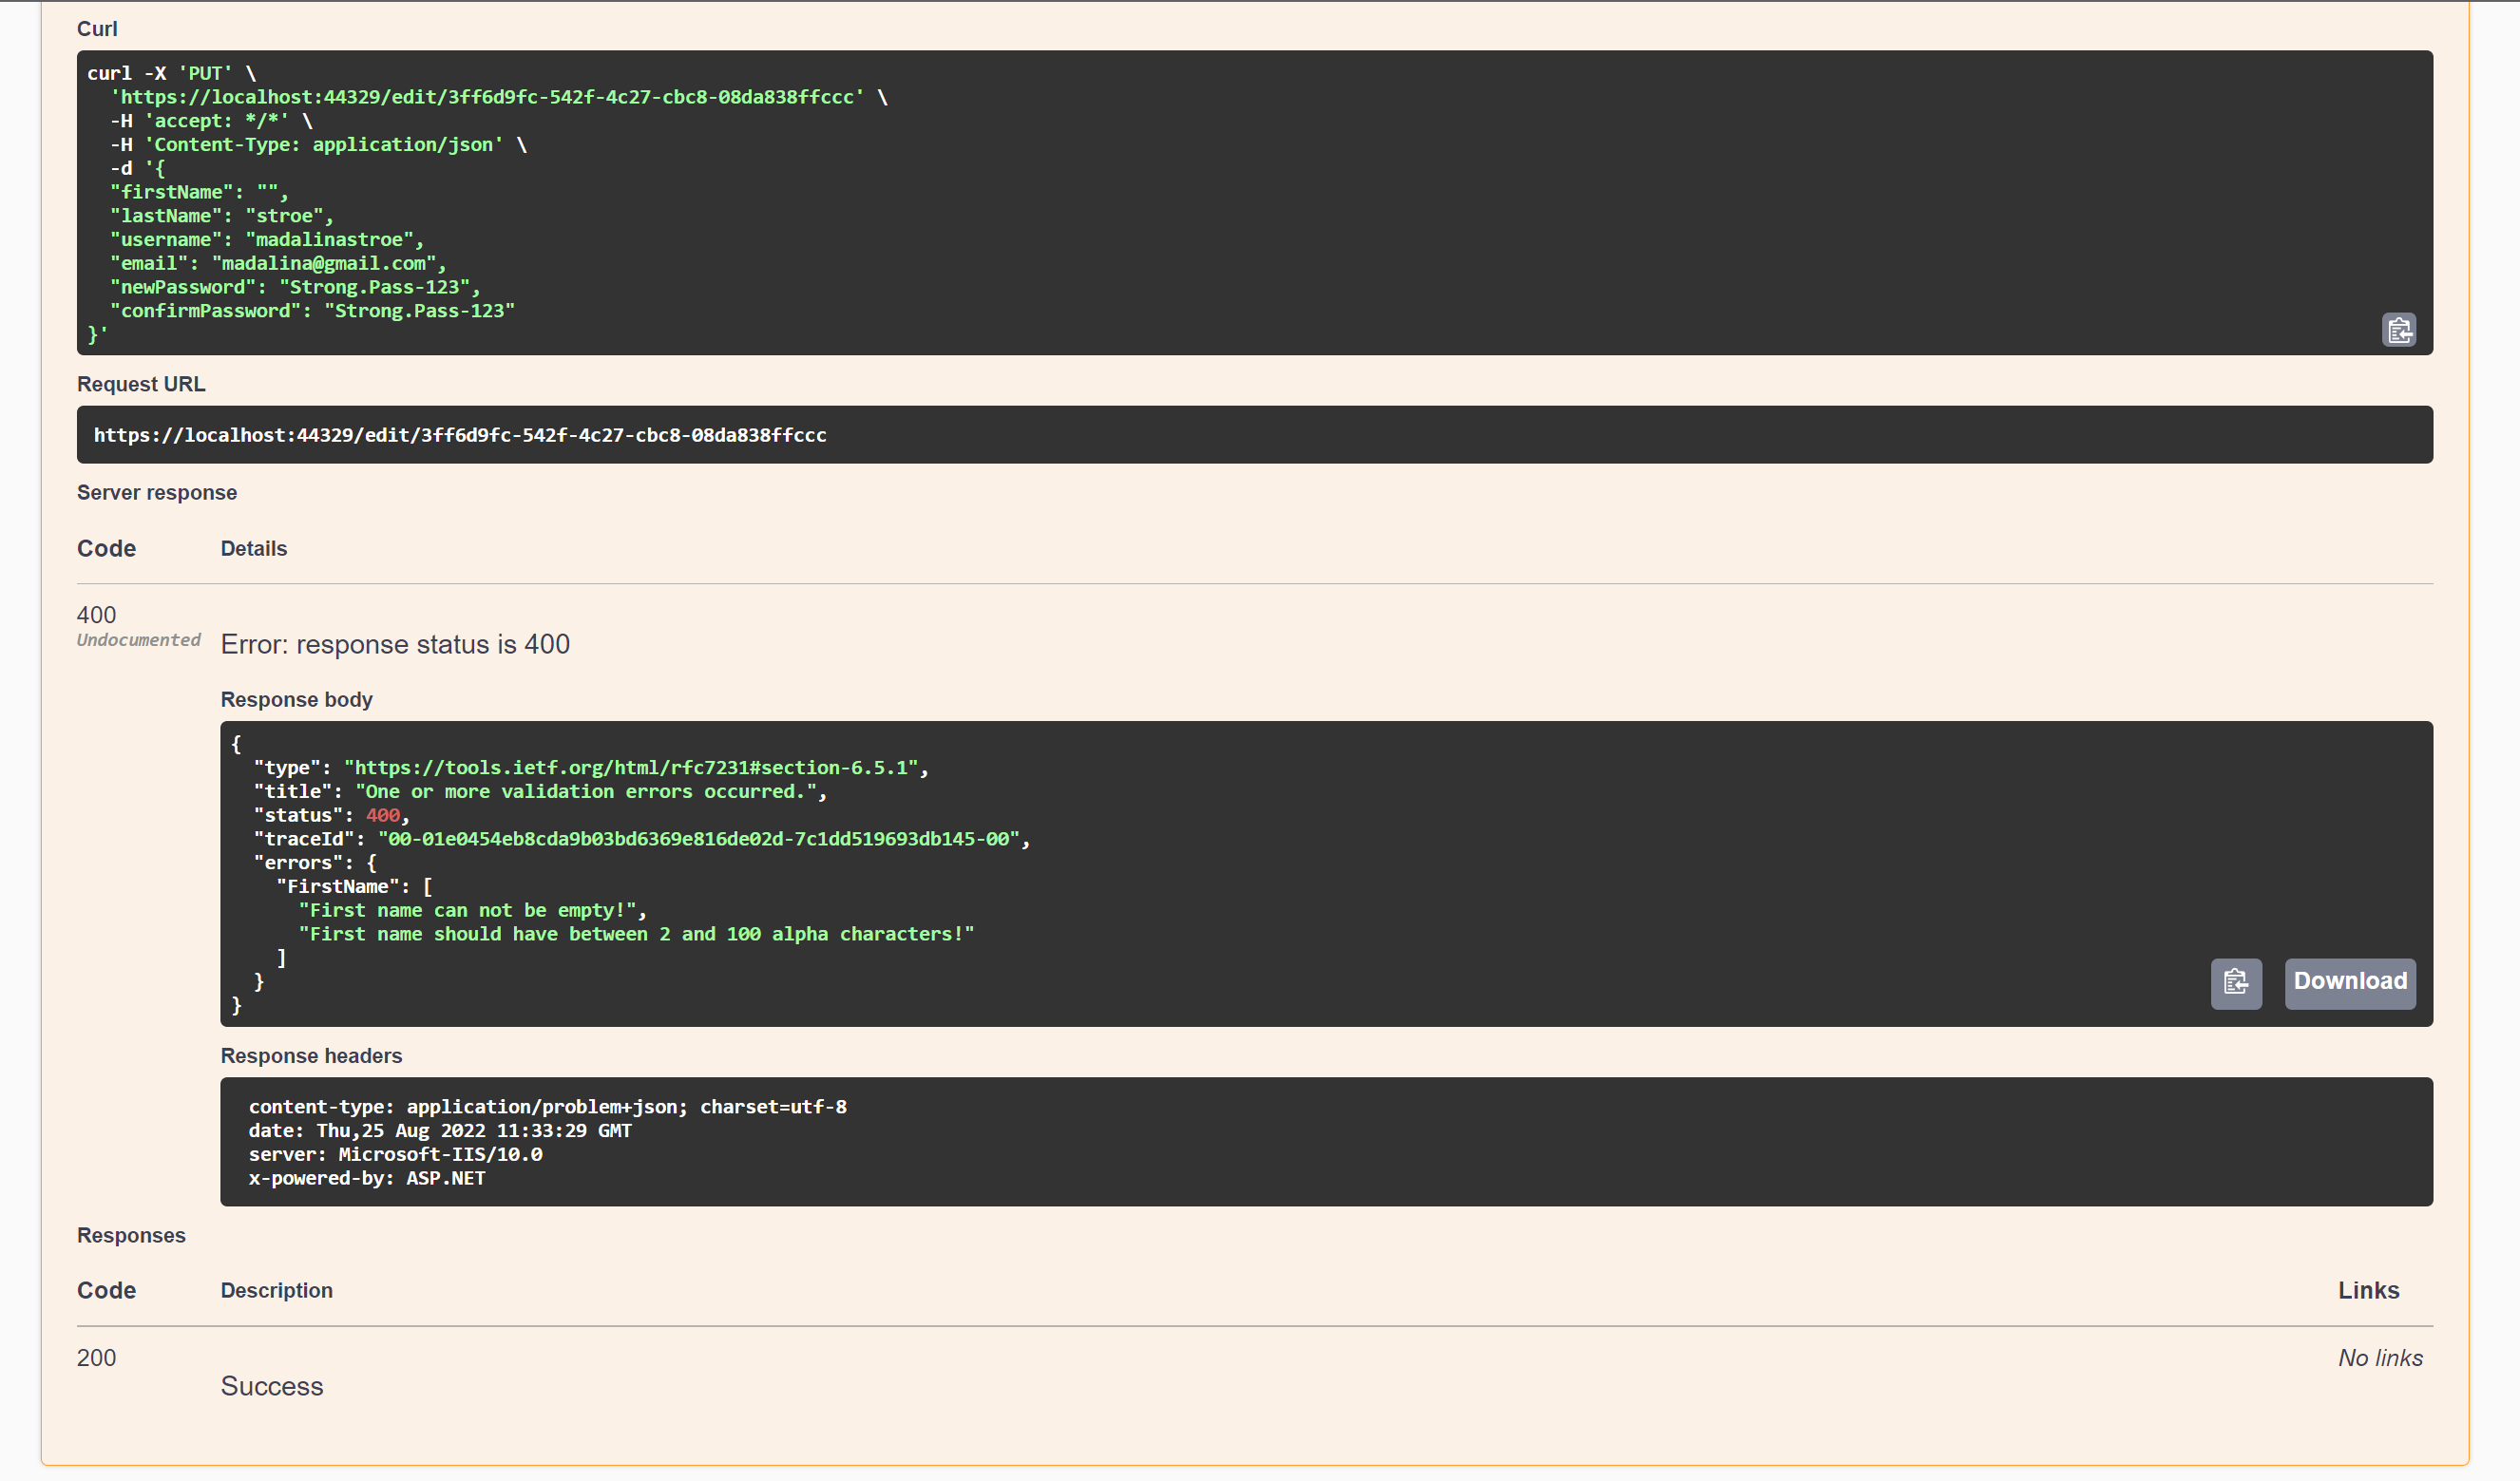
\includegraphics[width=100mm, scale=2]{figs/editWrong2.png}
    \caption{Response - Editare detalii personale când un câmp este gol}
	\label{fig:editWrong2}
\end{figure}


\section{Testare frontend}
Pentru partea de frontend, testarea s-a realizat manual, la nivelul fiecărei pagini, pentru a testa dacă funcționalitatea este cea așteptată în funcție de inputul utilizatorului.
Rezultatele se pot observa în figurile \ref{fig:testareFE1}, \ref{fig:testareFE2} și \ref{fig:testareFE3}.

\begin{figure}[h]
	\centering
	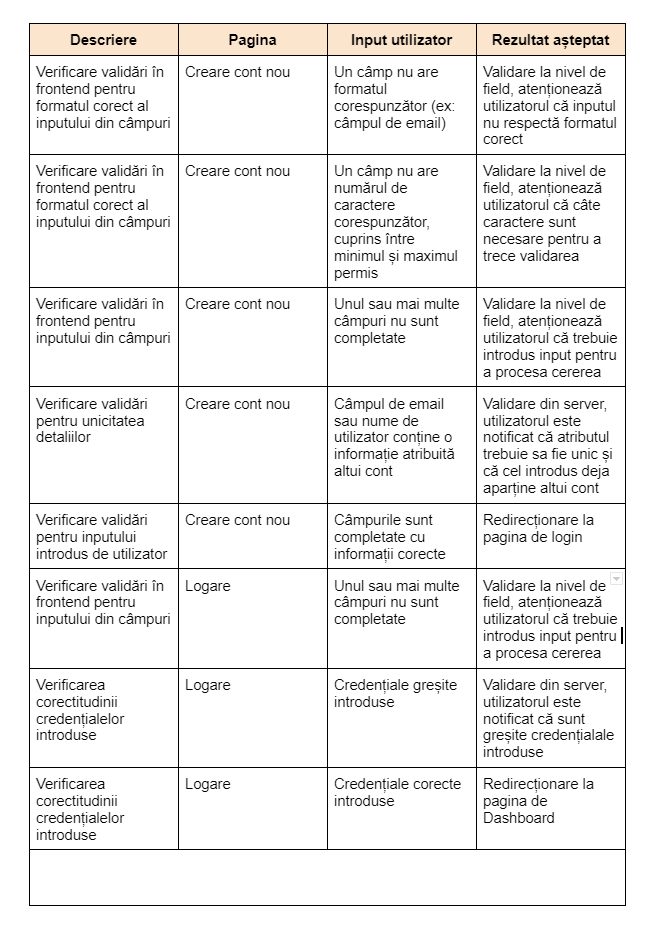
\includegraphics[height=100mm]{figs/testareFE1.png}
    \caption{Testare modul frontend - partea 1}
	\label{fig:testareFE1}
\end{figure}

\begin{figure}[ht]
	\centering
	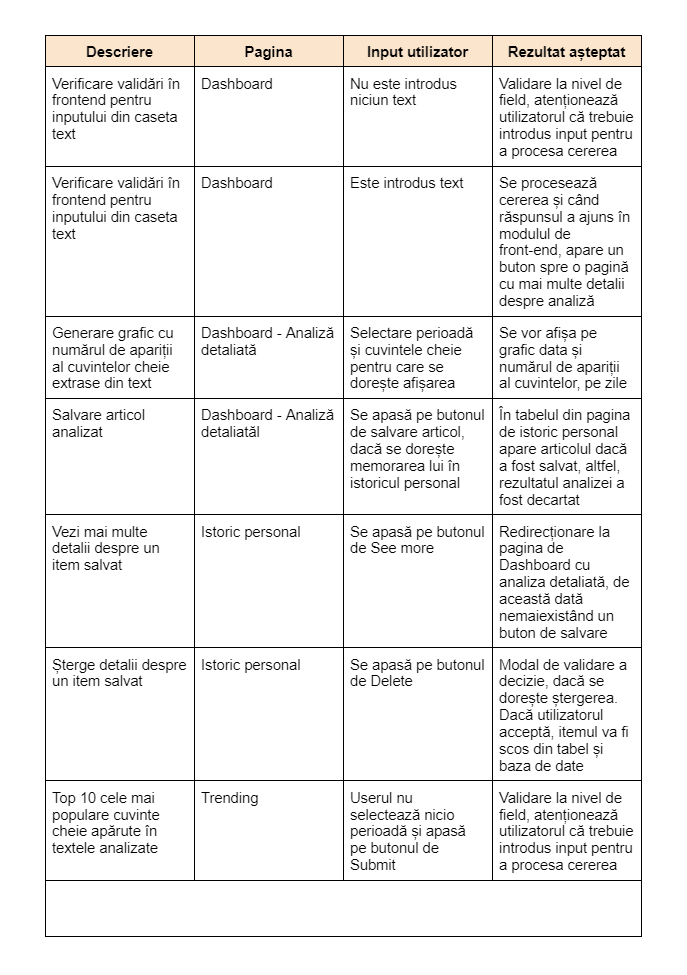
\includegraphics[height=100mm]{figs/testareFE2.png}
    \caption{Testare modul frontend - partea 2}
	\label{fig:testareFE2}
\end{figure}

\begin{figure}[ht]
	\centering
	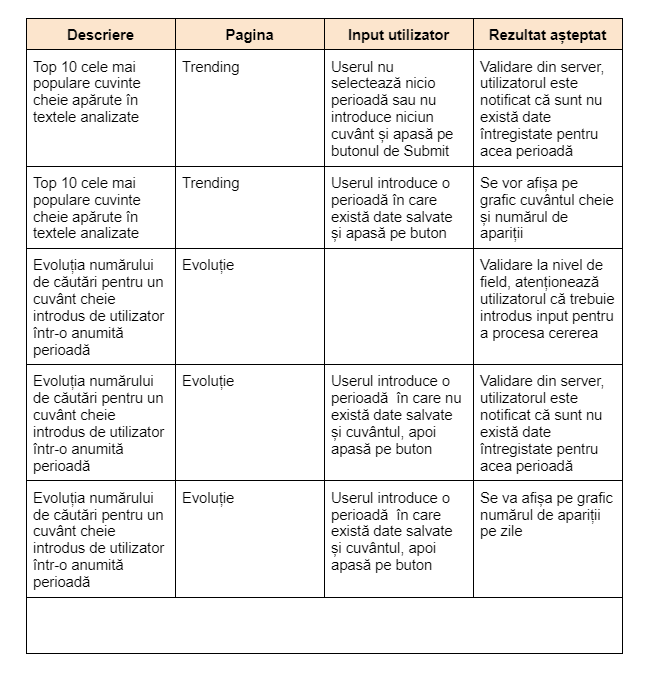
\includegraphics[height=100mm]{figs/testareFE3.png}
    \caption{Testare modul frontend - partea 3}
	\label{fig:testareFE3}
\end{figure}
\ \\
\section{Testare analiză a textului}
Pe partea de analiză de text, testarea s-a realizat prin compararea empirică a mai multor modele din Hugging Face utilizând diferite texte.